%!TEX root = ./main.tex
	\note{
        \begin{itemize}
        	\item Welkom!
            \item English?
        	\item Wat is HHGCS? 
            \begin{enumerate}
            	\item Praktische informatie over Unief
                \begin{itemize}
                	\item Waar boeken halen, wat is blackboard, ...
                \end{itemize}
                \item Praktische info i.v.m. de opleiding
                \begin{itemize}
                	\item Aangeven welke tools er zijn
                	\item Korte uitleg, zodat je je plan ermee kan trekken
                \end{itemize}
                \item Niet verplicht!
        	\end{enumerate} 
            \item Bedanking Mevr. Laenens :)
        \end{itemize}
	}
    
	\section{Intro}
    \addtocounter{minutes}{2}
	\begin{frame}
		\frametitle{Intro} 
		%\framesubtitle{}
        Initiatief van studenten
        
        \begin{figure}
        	\begin{minipage}{0.3\linewidth}
                \centering
            	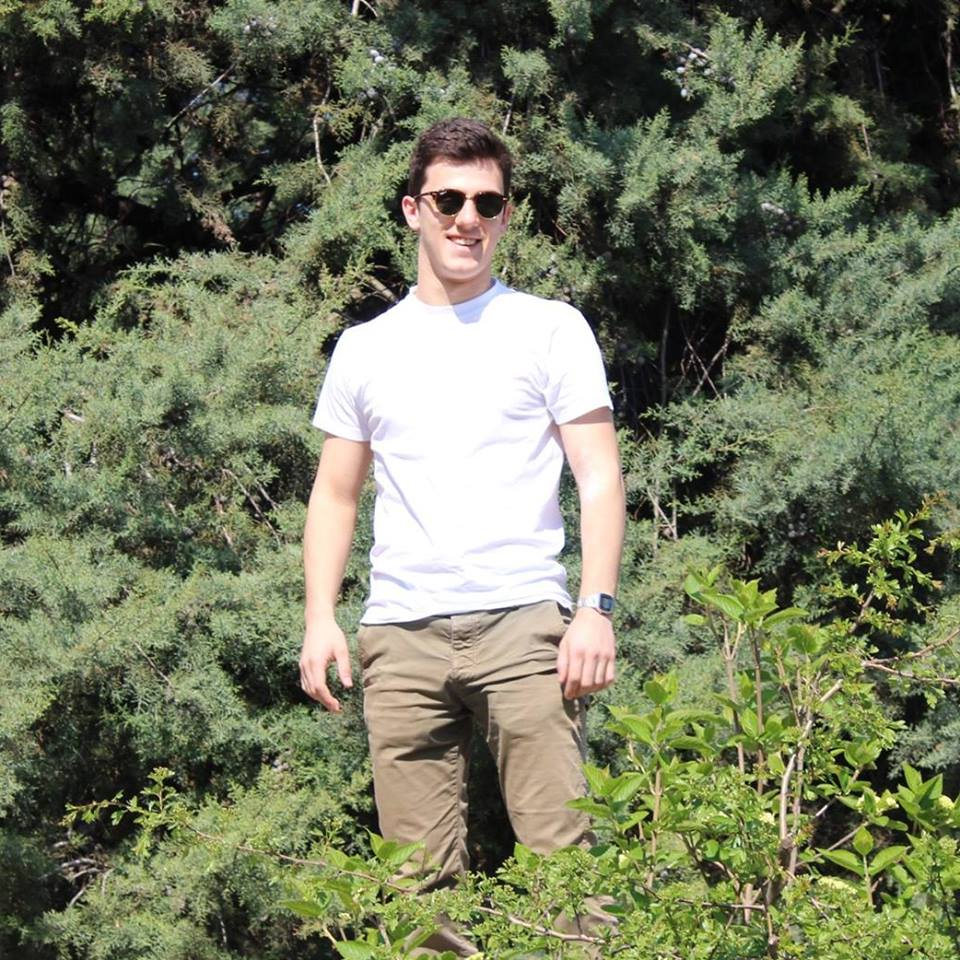
\includegraphics[width=\linewidth]{res/andrei} \\
            	\footnotesize Andrei Bondarenko
            \end{minipage}
            \begin{minipage}{0.3\linewidth}
            	\centering
				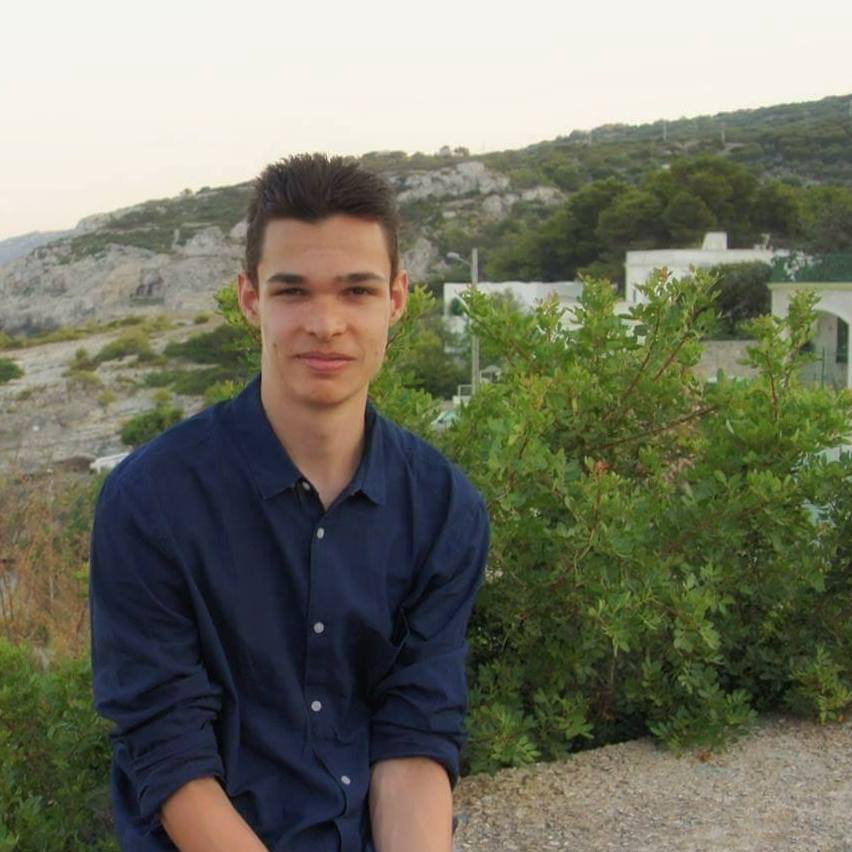
\includegraphics[width=\linewidth]{res/stijn} \\
            	\footnotesize Stijn Rosaer
        	\end{minipage}
            \begin{minipage}{0.3\linewidth}
            	\centering
				
\includegraphics[width=\linewidth]{res/igor} \\
            	\footnotesize Igor Schittekat 
        	\end{minipage}
            \begin{minipage}{0.3\linewidth}
            	\centering
				
\includegraphics[width=\linewidth]{res/joey} \\
            	\footnotesize Joey De Pauw
        	\end{minipage}
            \begin{minipage}{0.3\linewidth}
            	\centering
				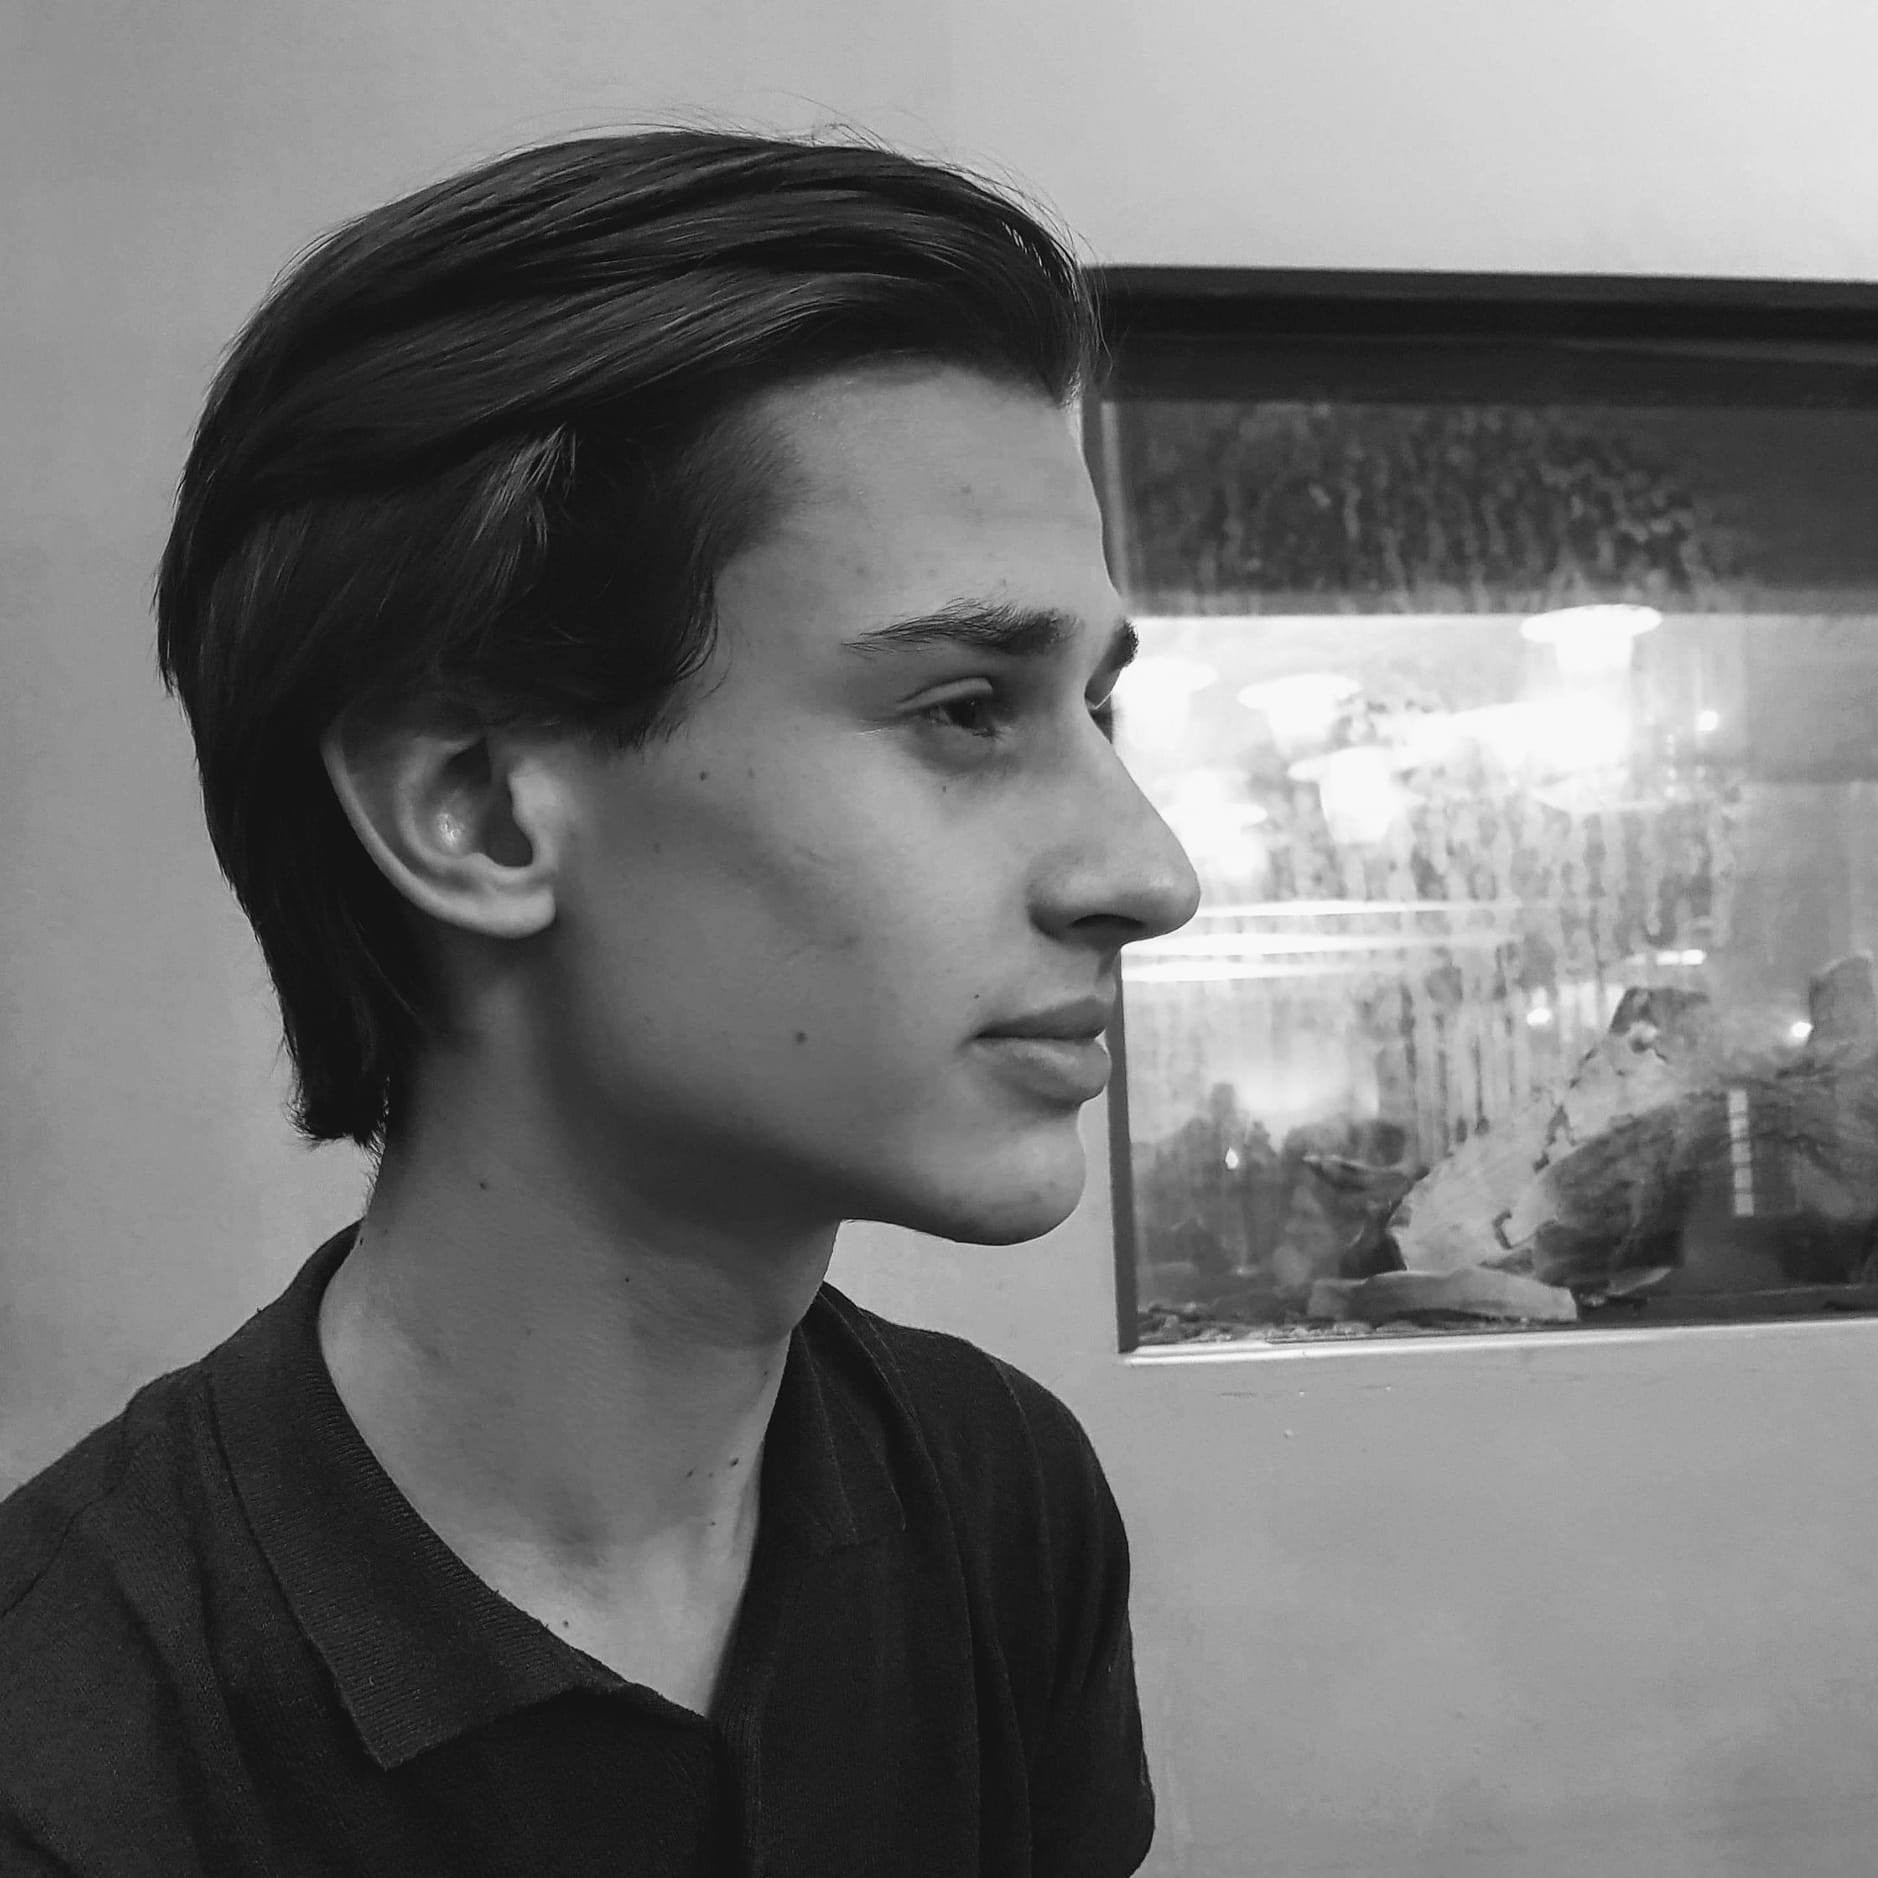
\includegraphics[width=\linewidth]{res/senne} \\
            	\footnotesize Senne Rosaer
        	\end{minipage}
            \begin{minipage}{0.3\linewidth}
            	\centering
				
\includegraphics[width=\linewidth]{res/toon} \\
            	\footnotesize Toon Meynen
        	\end{minipage}
        \end{figure}
        
        \note{
			Wij zijn allemaal bereikbaar. Spreek ons aan!
    	}
	\end{frame}  
   
    
    \section{Planning}
    \addtocounter{minutes}{3}
	\begin{frame}
		\frametitle{Planning}
        \includeSchedule
        
        \note{
        	\begin{itemize}
				\item Volgende sessie:  Dual boot $->$ USB stick en laptop
                \item Extra info? vraag het ons!
			\end{itemize}
        }
	\end{frame}
    
    \section{WINAK}
	\begin{frame}
		\frametitle{WINAK}
		\framesubtitle{\textbf{W}iskunde \textbf{I}nformatica \textbf{Na}tuurkunde \textbf{K}ring}
        
        \begin{itemize}
            \item\href{https://www.facebook.com/groups/140326299910429/}{Facebook Groep $\vcenter{\hbox{
\includegraphics[width=0.45cm]{res/link}}\vspace{0.1cm}}$}
            \item\href{http://www.winak.be/}{Forum $\vcenter{\hbox{
\includegraphics[width=0.45cm]{res/link}}\vspace{0.1cm}}$}
            \item\href{http://tuyaux.winak.be/}{Tuyaux $\vcenter{\hbox{
\includegraphics[width=0.45cm]{res/link}}\vspace{0.1cm}}$}
            \item Lidkaart
            \item Mentoren
            \begin{itemize}
            	\item Elise (Wiskunde)
            	\item Theumes (Fysica)
				\item Toon (Informatica)
			\end{itemize}
			\item Doop
            \item\href{https://www.facebook.com/events/278437369338614}{Openings Cafe Avond $\vcenter{\hbox{
\includegraphics[width=0.45cm]{res/link}}\vspace{0.1cm}}$}
            
		\end{itemize}

	\end{frame}
    
%     \section{Blackboard \& SiSa}
% 	\begin{frame}
% 		\frametitle{Blackboard}
% 		\framesubtitle{https://blackboard.uantwerpen.be}
%         \begin{itemize}
%         \item Facebook van de universiteit
%           \begin{itemize}
%             \item Updates
%             \item Projecten
%             \item Oefeningen
%           \end{itemize}
% 		\end{itemize}
% 	\end{frame}
	
% 	\begin{frame}
% 		\frametitle{SiSa}
% 		\framesubtitle{https://sisastudent.uantwerpen.be}
%         \begin{itemize}
%           \item Administratie van de universiteit
%           \begin{itemize}
%             \item Inschrijven
%             \item Lessenrooster
%             \item Rekeningen
%           \end{itemize}
% 		\end{itemize}
% 	\end{frame}
    
    \section{Email \& Lessenrooster}
	\begin{frame}
		\frametitle{Email}
		\framesubtitle{https://mail.student.uantwerpen.be}
        \begin{center}
        	\tcbox[colback=white, colframe=darkblue]{
            	\parbox{7.5cm}{
                  \centering
                  s018xxxx@ad.ua.ac.be OF \\
                  voornaam.achternaam@student.uantwerpen.be
                }
            }
        \end{center}
    	\textbf{IMAP (inkomend)}
        \begin{tabularx}{\linewidth}{rX}
          Server name & outlook.office365.com \\
          Port & 993 \\
          Encryption & SSL \\
		\end{tabularx} \vspace{0.5cm}
        
		\textbf{SMTP (uitgaand)}
        \begin{tabularx}{\linewidth}{rX}
          Server name & smtp.office365.com \\
          Port & 587 \\
          Encryption & STARTTLS \\
		\end{tabularx} \vspace{0.5cm}

        
        \note{
        	Note: mogelijk dient u poort 143 te gebruiken bij de IMAP instellingen, wanneer het niet meteen lukt om met bovenstaande gegevens uw e-mail binnen te halen.
        }
	\end{frame}
    
	\begin{frame}
		\frametitle{Lessenrooster}
		%\framesubtitle{}
        \begin{itemize}
       	  \item SiSa $\rightarrow$ rooster $\rightarrow$ abonneer op rooster
          \item Agenda toevoegen via url
        \end{itemize}
	\end{frame}
    
    \section{Cursusdienst \& Printen}
	\begin{frame}[allowframebreaks=10]
		\frametitle{Cursusdienst}
		%\framesubtitle{}
        \href{https://www.uantwerpen.be/nl/onderwijs/studerenuantwerpen/starten-als-student/colleges-cursussen-examens/cursusdienst/}{Website UA - Cursusdienst $\vcenter{\hbox{
\includegraphics[width=0.45cm]{res/link}}\vspace{0.1cm}}$} \\ \vspace{1cm}
        Tips:
        \begin{itemize}
            \item Verplicht $\neq$ Verplicht Verplicht
            \item Cursussen zeker kopen
            \item Handboeken ter referentie
            \item Schrijf de nummers van de cursussen en handboeken op
		\end{itemize}
        
        \note{
            \begin{itemize}
                \item Verplicht = sterk aangeraden door prof
                \item Cursussen: relatief goedkoop, soms op examens gebruiken
                \item Handboeken: duurder, meer achtergrond info, kan handig zijn
            \end{itemize}
        }
        
        \framebreak
        \begin{figure}
        	\centering
            \vspace*{0.02cm}
            \textbf{Campus Groenenborger} \\
            \vspace{0.3cm}
        	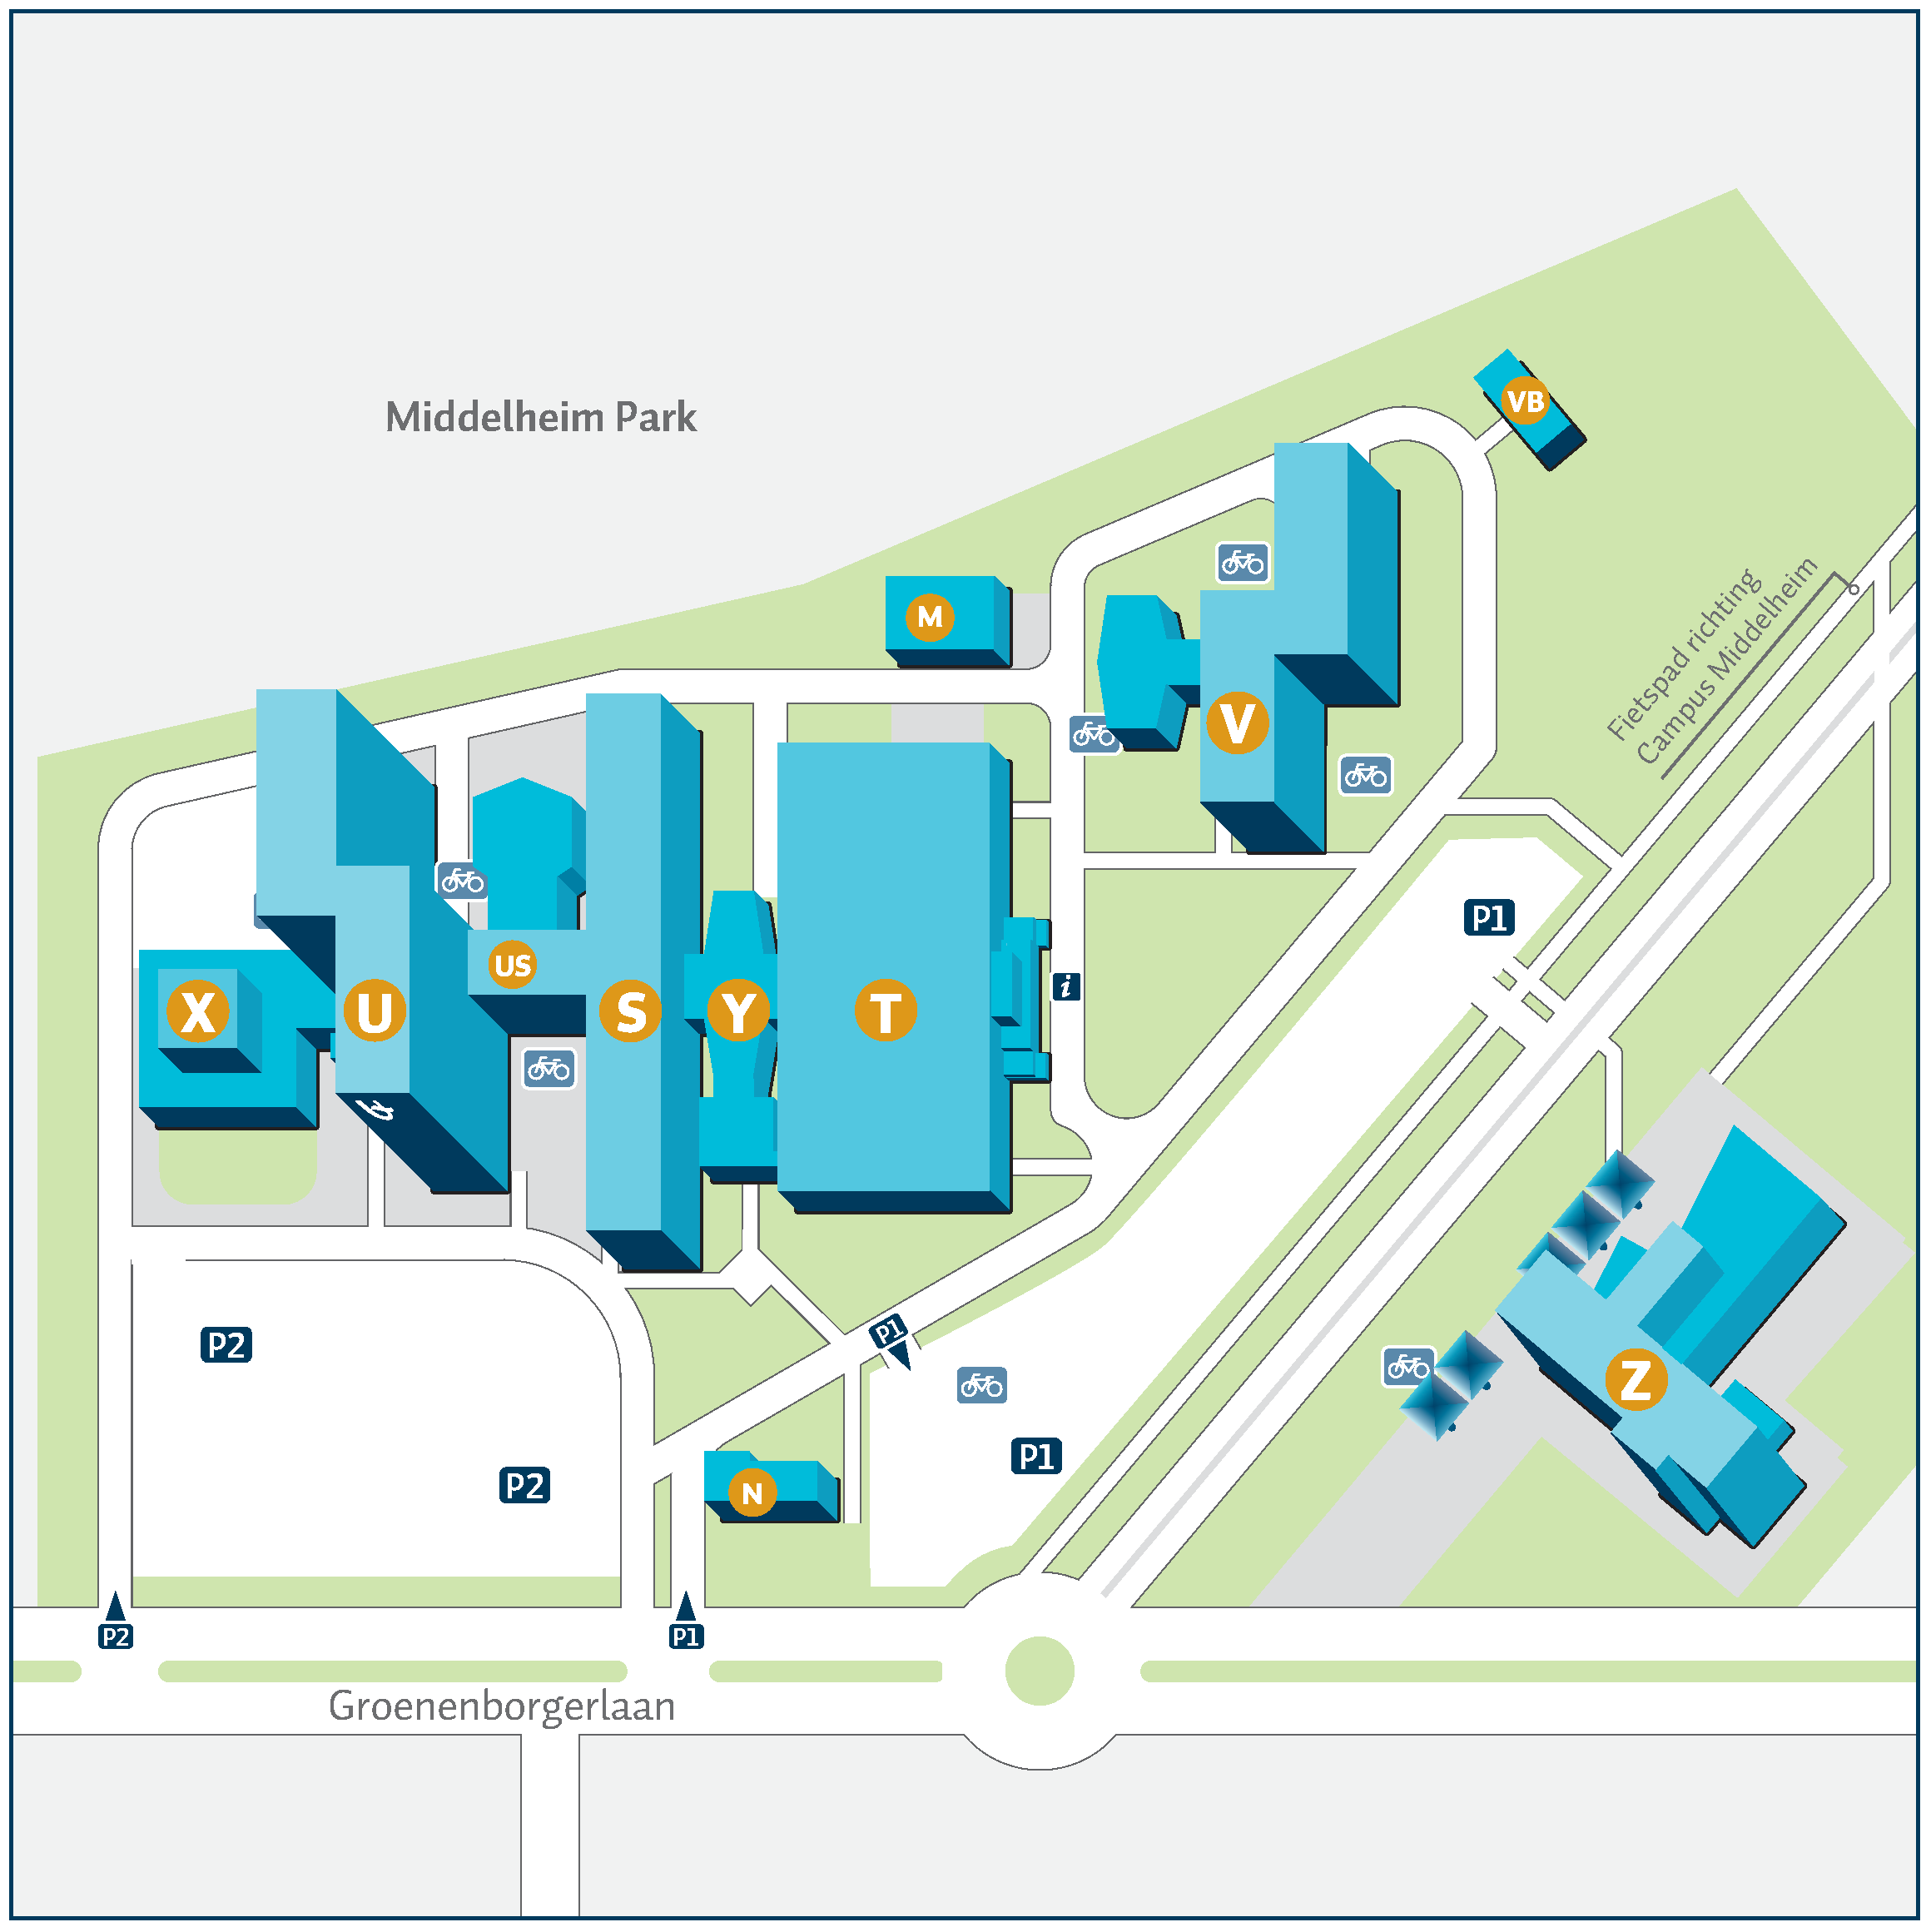
\includegraphics[width=0.65\linewidth]{res/CGB}
        \end{figure}
        \framebreak
        \begin{figure}
        	\centering
            \vspace*{0.02cm}
            \textbf{Cursusdienst Campus Groenenborger U027} \\
            \vspace{0.3cm}
       		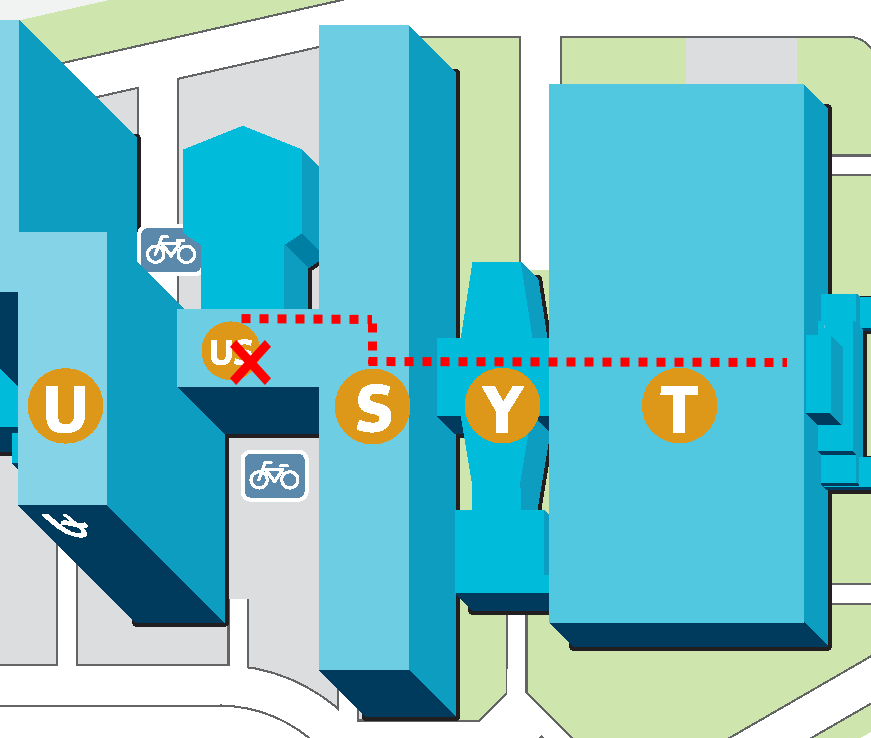
\includegraphics[width=0.8\linewidth]{res/CGB_CD_small}
        \end{figure}
	\end{frame}
    
	\begin{frame}[allowframebreaks=10]
		\frametitle{Printen}
		% framesubtitle{}
        \href{https://www.uantwerpen.be/nl/bibliotheek/diensten/faciliteiten/ter-plaatse/printen-kopieren-scannen/}{Website UA - Printen $\vcenter{\hbox{
\includegraphics[width=0.45cm]{res/link}}\vspace{0.1cm}}$} \vspace{1cm}
        \begin{enumerate}
        	\item Printkaart kopen
            \item Printkaart opladen (online)
            \item Studenten account koppelen aan kaart
            \item Printen
        \end{enumerate}
%         \framebreak
%         \begin{figure}
%         	\centering
%             \vspace*{0.02cm}
%             \textbf{Bibliotheek Campus Groenenborger} \\
%             \vspace{0.3cm}
%        		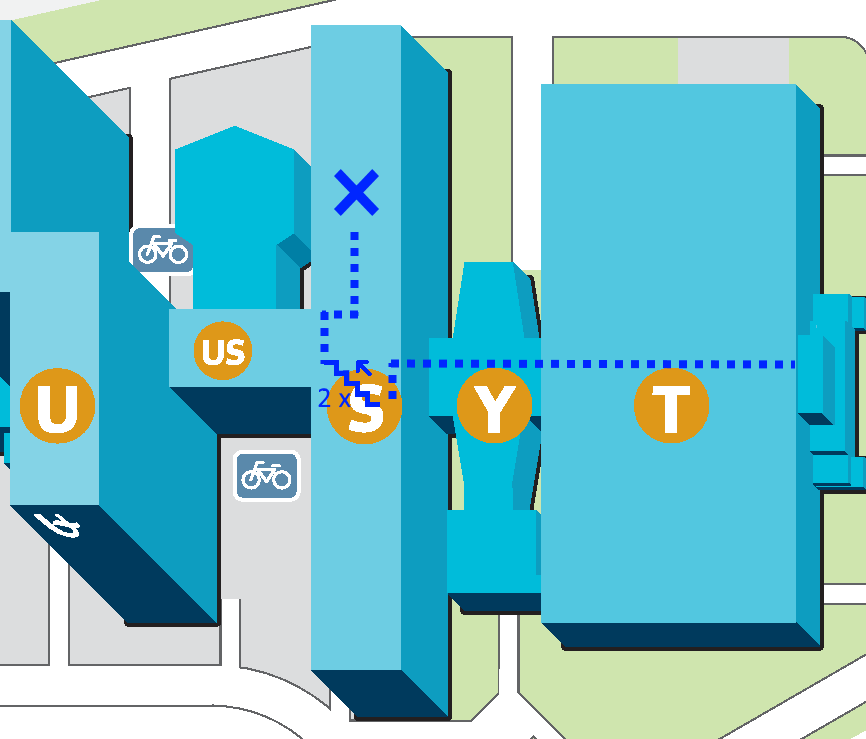
\includegraphics[width=0.8\linewidth]{res/CGB_BIB_small}
%         \end{figure}
	\end{frame}
    
    \section{Rondleiding \& Receptie}
	\begin{frame}
		\frametitle{Rondleiding \& Receptie}
		\framesubtitle{Sponsored by WINAK}
        \begin{itemize}
        	\item Gebouw G
            \item Leercentrum ``De Parabool''
            \item PC Labo
            \item Free Drinks
		\end{itemize}
	\end{frame}
